

\documentclass{article}
\usepackage{graphicx}
\graphicspath{ {./images/} }


\begin{document}

\title{IoT Based Expert System for Diabetes Diagnosis and Insulin
Dosage Calculation}
\author{Nandhini}
\maketitle

\section{ Introduction}

IoT encompassing advanced technologies such as wireless sensor networks (WSN), artificial intelligence,
and cloud computing plays an important role in many domains comprising of robotics, logistics, transportation, and
health-care.

Advances in wireless sensor networks (WSN) have created an innovative ground for e-health and wellness application development. The new initiatives tend to be integrated into the patient information ecosystem instead of being separated into monitoring and decision processes. There are potential benefits to ageing population, where elderly people could be monitored and treated at the comfort of their own homes.

In 2012, over 1.5 million people died because of diabetes and there is still no known permanent cure for the disease. Fully autonomous health monitoring wireless systems can have many useful applications including glucose level measurement for diabetics. CGM equipped with alarm systems can help patients to take corrective action(s) such as decisions on their diet, exercise and when to take medication.
In this paper, the presented work aims to study the feasibility of invasive and secure CGMS using IoT. The work is to design an IoT-based system architecture from a sensor device to a back-end system for presenting real-time glucose, body temperature and contextual data. In summary, the main contributions in this paper are as follows:

\begin{itemize}

 \item proposing continuous glucose monitoring IoT-based system.
 \item designing an energy efficient sensor device using nRF protocol.
 \item designing an energy harvesting unit for the sensor device to extend the sensor device’s battery life.
\end{itemize}

\section{Related works}

Many research applications in glucose monitoring are not based on IoT-based architectures. Correspondingly, doctors and caregivers cannot monitor glucose levels remotely in real-time. Murakami et al. 5 present a CGM system in critical cardiac patients in the intensive care unit. Glucose data is transmitted via BLE to a PDA (smart-phone, or Ipad) for visualization.
A team of researchers have developed an advanced IoT-based system for real-time and remote continuous monitoring of glucose, contextual data, and body temperature. The sensor devices are integrated with an energy harvesting unit, a power management unit and ultra low-energy nRF wireless communication, as well as dedicated gateways equipped with advanced services such as push-notification in the event of an abnormality.

\section{ System Architecture}
. System architecture
In the furtherance of providing continuous glucose monitoring in real-time locally and remotely, the CGMS architecture shown in Fig .1 is based on an IoT architecture. The system includes three main components such as a portable
sensor device, a gateway and a back-end system.

\begin{center}
  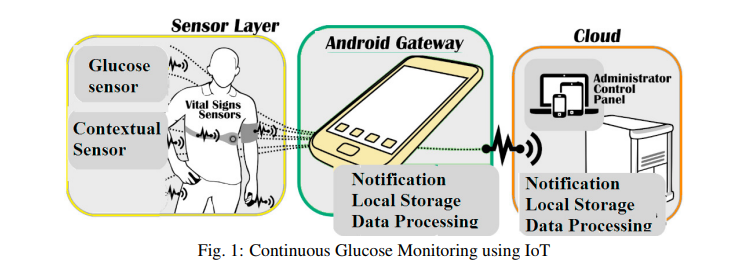
\includegraphics[scale=0.5]{sys arch.png}
  \label{fig:sys}
\end{center}

\subsection{Sensor device structure}
The sensor device whose structure is shown in Fig.2 consists of primary component blocks such as sensors, a microcontroller, a wireless communication block, energy harvesting and management components. In the device, the micro-controller receives glucose data from an implantable glucose sensor while it collects environmental and body temperature via data link wires such as UART, SPI or I2C.
The nRF wireless communication block is responsible for transmitting data from the micro-controller to the gateway. The block includes a RF transceiver IC for the 2.4GHz ISM band and an embeddedantenna. Due to 2Mbps supporting, nRF completely fulfills the requirements of transmission data rates in a CGM system.


\begin{center}
  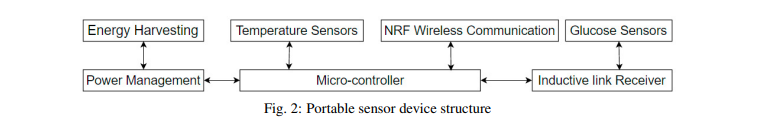
\includegraphics[scale=0.5]{sensor.png}
  \label{fig:sen}
\end{center}

\subsection{Energy harvesting unit}
To power the glucose sensor node a combination of ambient and human powered sources is selected. Due to its ubiquitous availability RF energy is an adequate source for this application.
Energy harvesting refers to harnessing energy from the environment or other energy sources (body heat, foot strike, finger strokes) and converting it to electrical energy. If the harvested energy source is large and periodically or continuously available, a sensor node can be powered perpetually. Energy sources can be broadly classified into the following two categories:

(i) Ambient Energy Sources: Sources of energy from the surrounding environment, e.g., solar energy, wind energy and RF energy, and 

(ii) Human Power: Energy harvested from body movements of humans. Passive human power sources are those which are not user controllable like blood pressure, body heat and breath. 


\begin{center}
  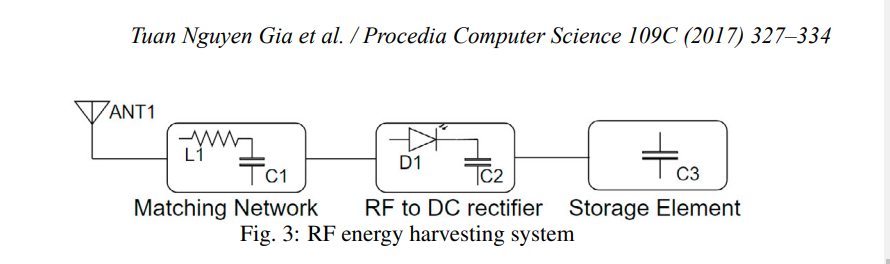
\includegraphics[scale=0.5]{rf.png}
  \label{fig:rf}
\end{center}

Active human power sources are those that are under user control, and the user exerts a specific force to generate the energy for harvesting, e.g., finger motion, paddling and walking. To power the glucose sensor node a combination of ambient and human powered sources is selected. Due to its present availability, RF energy is an adequate source for this application. Also, since the sensor is mounted on the human body it makes sense to exploit this medium as a source of energy. Through the use of a Thermoelectric Generator (TEG), thermal energy can be converted into electrical energy. 


\begin{center}
  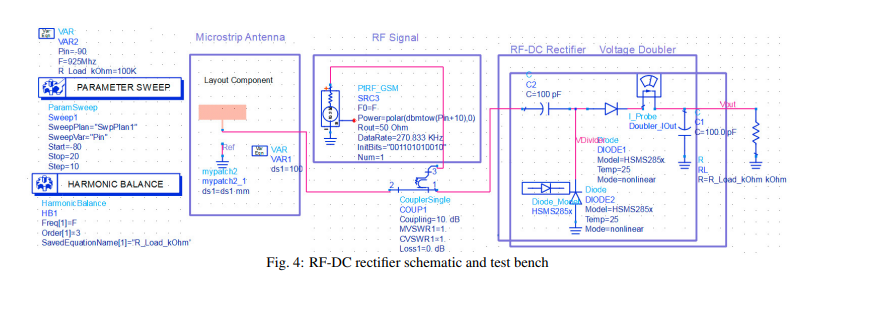
\includegraphics[scale=0.5]{rf-dc.png}
  \label{fig:rfdc}
\end{center}


\begin{center}
  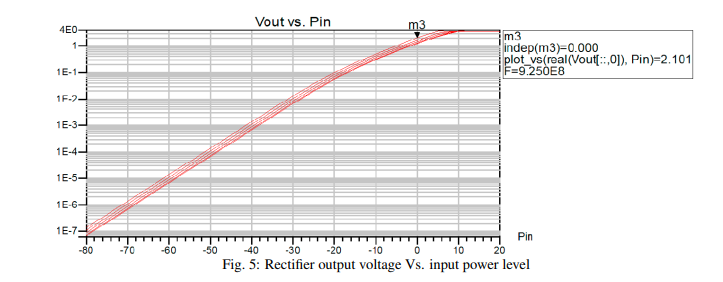
\includegraphics[scale=0.5]{vs.png}
  \label{fig:vs}
\end{center}


\subsubsection{ power management unit}
In battery powered wireless sensor network, the sensor goes to the idle status to prevent power draining. In case the sensor receives an incoming message (packet), the sensor should go from idle to active status. Dutycycling is an efficient approach that reduces idle-mode power consumption.
k. The power management system is composed of both a radio-triggered wake-up circuit and a voltage sensor.The wake-up circuit is implemented using a low-power Schmitt trigger circuit. The voltage sensor is implemented using a differential amplifier with positive feedback.

\subsection {  Gateway and back-end structure }
The gateway collects data from wireless sensor devices and transmits the data to Cloud servers. The gateway performs its tasks by using an nRF transceiver and a wireless IP-based transceiver (i.e. Wifi, GPRS or 3G). The nRF transceiver, which is a plug-able component, is compatible with all types of smart devices (i.e. Android, iPhone, tablet). The nRF transceiver consists of a micro-controller and a low power RF transceiver IC, and an FTDI component. The micro-controller and the nRF components are the same as the ones used in the sensor device. The FTDI chip is used for converting from a UART connection to a USB connection. In addition to mentioned tasks, the gateway provides advanced services such as data processing, local database, local host with user interface and push notification. Due to a small amount of collected data (4-8 samples per 10 minutes), local databases can store the data for a long period of time. By supplying a local host with a user interface, real-time data can be monitored directly from the gateway without requiring Cloud servers. This helps to eliminate an unnecessary latency of transmitting and receiving data to and from the Cloud, respectively. In the gateway, decision making and push notification services work together to provide real-time notifications to doctors or caregivers. For example, when a monitored glucose level is higher and lower than an acceptable level, the decision making service triggers the push notification to send messages for notifying a doctor in real-time. The back-end part comprises Cloud and a user access terminal. Doctors can access real-time data in Cloud remotely via a web browser or a mobile application.  

\begin{center}
  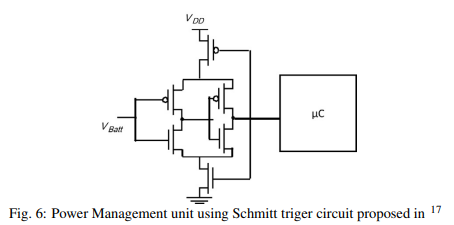
\includegraphics[scale=0.5]{sch.png}
  \label{fig:sch}
\end{center}


\begin{center}
  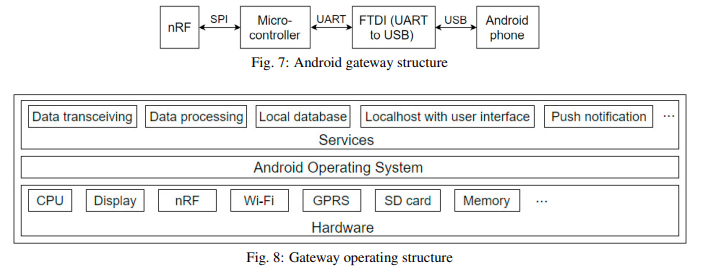
\includegraphics[scale=0.5]{back-end.png}
  \label{fig:back}
\end{center}


An Android app is built in the gateway for receiving data from the nRF component and performing other services. When data is available at one end of the USB port, the app automatically reads the data and performs the data processing service. In addition, the app is capable of representing the processed data in text and graphical forms and triggering a push notification service. 


The push notification service is implemented by a push notification API. When the mobile app detects abnormal situations (i.e. too low or too high glucose level), the push notification service in the gateway is triggered for sending notification messages to Cloud which then notifies doctors and an end-user wearing the sensor device. 


\section{ Implementation}
To evaluate the feasibility of the CGM system using IoT, the entire system is executed. Initially, the interaction of the biological tissue under investigation is studied. Since the glucose sensor will be subcutaneous, the electrical characteristics of the biological tissue i.e. skin will be evaluated from which the amount of power loss and absorption due to propagation through the biological tissue will be estimated. It is imperative to make sure that subjecting the human body to these continuous signals is within the safe specified measures. The guidelines for

Electromagnetic Field Exposure (EMF) is in terms of Specific Absorption Rate (SAR) and the equivalent plane wave power density (SW/m2). SAR is a measure of the rate of energy absorption per unit mass due to exposure to an RF source. SAR is defined as :
\begin{equation}
    SAR = \frac{(effErms^2 )}{(W/Kg)} 
\end{equation}
 

Where eff is the effective conductivity of the biological material such as skin and is proportional to the frequency of the applied field, is the mass density which is approximately 1000 kg/m3 for most biological tissues, and Erms is the root-mean-square value of the electric field E at the measurement point. As specified in the operating frequency of 2.4 GHz, the maximum E and S are 61 V/m and 10 W/m2 respectively which are well below the targeted operation power of the wireless sensor node.   

\section{Conclusion}
In this paper, we presented a real-time remote IoT-based continuous glucose monitoring system. Through the system, doctorsand caregivers can easily monitor their patient anytime, anywhere via a browser or a smart-phone application. Sensor nodes are able to obtain several types of data (i.e. glucose, body temperature, and environmental data) and transmit the data wirelessly to the gateway efficiently in term of energy consumption.

\section{References}
\begin{itemize}
\item IoT-based continuous glucose monitoring system: A feasibility study
\item https://www.copperpodip.com/post/iot-based-glucose-monitoring-systems
\item An IoT-Based Glucose Monitoring Algorithm to
Prevent Diabetes Complications.
\end{itemize}

\end{document}

